\setcounter{chapter}{2}

\chapter{Coalition Formation for Autonomous Web Services}

\section{Preliminaries}\label{s:preliminaries}

In this section, we discuss the parameters and preliminary
concepts that we use in the rest of the paper.

\subsection{The Architecture}

Our system consists of three main types of entities working
together:

\emph{1) Web services} are rational entities\footnote{The term
rational is used here in the sense that web services are utility
maximizers} providing services to end users. They aim to maximize
their individual income by receiving enough requests from end
users. In order to increase their revenue, web services seek for
more tasks if they have the capacity and throughput to do so. Web
services can join communities to have better efficiency by
collaborating with others, to have access to higher market share,
and to have opportunity of receiving a bigger task pool from end
users. Throughout this paper, in
our equations, we refer to web services as $ws$ and to the set of
web services hosted by a given community as $C$. To simplify the
notation, sometimes we simply write $ws$ instead of $ws \in C$ to
go through the elements $ws$ of the set $C$.

\emph{2) Master Web Services} or the community coordinators, are representatives of the
communities of web services and responsible for their management.
Communities receive requests from users and aim to host a healthy
set of web services to perform the required tasks. They seek to
maximize user satisfaction by having tasks accomplished according
to the desired QoS. In fact, higher user satisfaction will bring
more user requests and increase the market share and revenue of
the community.

\emph{3) Users} generate requests and try to find the best
available services. User satisfaction is abstracted as function of
quantity and quality of tasks accomplished by a given service.
Higher user satisfaction leads to higher trust of the community by users hence directing more requests towards that service provider.

\subsection{Web Service Parameters}\label{ws_parameters}

Web services come with different quality of service parameters.
These parameters with a short description are listed in Table
\ref{qosws}.

\begin{table}[!t]
\centering
\caption{List of web service QoS parameters.}
\begin{tabular}{|c|c||c|c|}
\hline
\textbf{Parameter} & \textbf{Definition} \\
\hline\hline
$Availability$ & Probability of being available during \\
&a time frame \\
$Reliability$ & Probability of successfully handling \\
&requests during a timeframe\\
$Successability$ & Rate of successfully handled requests \\
$Throughput$ & Average rate of handling requests \\
$Latency$ & The average latency of services\\
$Capacity$ & Amount of resources available\\
$Cost$ & Mean service fee \\
$Regulatory$ & Compliance with standards, law and rules\\
$Security$ & Quality of confidentiality \\
&and non-repudiation\\
\hline
\end{tabular}
\label{qosws}
\end{table}


We adopted a real world dataset \cite{DBLP:conf/smc/Al-MasriM09a}
which has aggregated and normalized each of these parameters to a
real value between 0 and 1. Since requests are not shared among
web services and are distributed among all of them inside a
community, each one of them comes with a given QoS denoted by
$(QoS_{ws})$. We assume that $(QoS_{ws})$ is obtained by a certain
aggregation function of the parameters considered in Table
\ref{qosws}. We use this quality output later in evaluating the
community \emph{worth} or \emph{payoff} function.

\subsection{Web Service Communities}\label{webservice-communities}

Figure \ref{fig_community} represents the architecture of web service communities. The communities are essentially an abstract model of web services. They aggregate web services and communicate with other entities such as UDDI registries and users, using identical protocols as web services. Web services join communities to increase their utility by having a larger market share and task pool. Community coordinators or master web services are responsible for community development, managing membership requests from web services and distributing user tasks among the community members. Community coordinators try to attract quality web services and keep the community as stable and productive as possible to gain better reputation and user satisfaction which results in having a higher market share for the community. The way the web services reside inside communities and how communities of web services are engineered is described comprehensively in \cite{DBLP:journals/ijebr/MaamarSTBB09}.

\begin{figure*}[!t]
\centerline{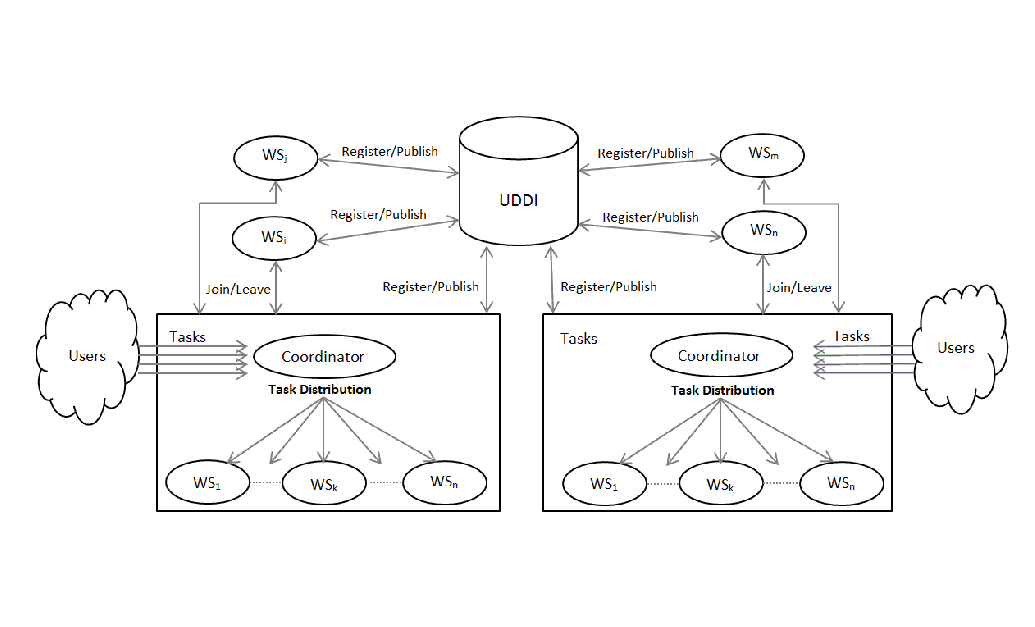
\includegraphics[width=15cm]{Figures/community.eps}}
\caption{Architecture of Web Service communities}
\label{fig_community}
\end{figure*}

\subsection{Cooperative Game Concepts}
Cooperative game is a branch of game theory that studies
strategies of self-interested entities or agents in a setting
where those agents can increase their payoff by binding agreements
and cooperating in groups. We let $N$ be a set of players. Any
subset $S$ of $N$ can form a group called $coalition$. A
\emph{coalitional game} is a pair $G = (N, v)$, where $v$ is called
a \emph{characteristic function} $v: 2^N \to \mathbb{R}$, mapping the set of players of the
coalition to a real number $v(S)$, the worth of $S$. This number
usually represents the output or payoff or again the performance
of these players working together as coalition.  If a coalition
$S$ is formed, then it can divide its worth, $v(S)$ in any
possible way among its members. The payoff vector $x \in
\mathbb{R}^S$ is the amount of payoff being distributed among the
members of the coalition $S$. The payoff vector satisfies two
conditions:

\begin{itemize}
    \item $x_i \geq 0$ for all $i \in N$, and
    \item $\sum_{i \in S} x_i \leq v(S)$
\end{itemize}

The second criteria is called the \emph{feasibility} condition,
according to which, the payoff for each agent cannot be more than
the coalition total gain. A payoff vector is also \emph{efficient}
if the payoff obtained by a coalition is distributed amongst the
coalition members: $\sum_{i \in S} x_i = v(S)$. This definition of
the characteristic function works in \emph{transferable utility}
(TU) settings, where utility (i.e., payoff) is transferable from
one player to another, or in other words, players have common
currency and a unit of income that is worth the same for all players
\cite{myerson1991game}.

When dealing with cooperative games, two issues need to be
addressed:\\ 1. Which coalitions among all possible coalitions to form? \\
2. How to reward each member when a task is completed?\\
%
The following definitions help address these two issues.

{\bf Definition 1 (Shapley value)} Given a cooperative game $(N,
v)$, the \emph{Shapley value} of player $i$ is given
by\cite{shapley_value}:
\begin{equation}\label{eq:shapley}
\phi_i(N,v) = \sum_{S \subseteq N \backslash \left\{i\right\} }
\frac{|S|! (|N|-|S|-1)!}{|N|!} (v(S \cup \left\{i\right\}) - v(S))
\end{equation}

\emph{Shapley value} is a unique and fair solution concept for
payoff distribution among the members of the coalition. It
basically rewards members with the amount of marginal contribution
they have to the coalition.

%\subsubsection{Core}

{\bf Definition 2 (Core)} A payoff vector $x$ is in the $core$ of
a coalitional game $(N, v)$ if and only if:
\begin{equation}\label{eq:core}
\forall S \subseteq N, \sum_{x_i \in S} x_i \geq v(S)
\end{equation}

The core is basically a set of payoff vectors where no subset of
players $S^\prime$ could gain more than their current payoff by
deviating and making their own coalition $\sum_{i \in S^\prime}
x_i \geq v(S^\prime)$. The sum of payoffs of the players in any
sub-coalition $S$ is at least as large as the amount that these
players could earn by forming a coalition by their own. In a
sense, it is analogue to Nash equilibrium, except that core is
about deviations from groups of entities. The core is the
strongest and most popular solution concept in cooperative game
theory. However, its computation is a combinatorial problem and
becomes intractable as the number of players increases. The core
of some real-world problem games may be empty, which means having
the characteristic function of the game $(N,v)$, there might be no
possible distribution of payoff assuring stability of subgroups.

{\bf Definition 3 (Convex cooperative games)} A game $(N,v)$ with
characteristic function $v(S)$ is convex if:
\begin{equation}\label{eq:convex}
v(S) + v(T) \leq v(S \cup T) + v (S \cap T), \forall S,T \subseteq
N.
\end{equation}

According to a classic result by Shapley \cite{S1971cores}, convex
games always have a non-empty core. We will use a variation of
convexity condition in our algorithm to check whether our
coalitions are stable.

\subsubsection*{$\epsilon$-core}\label{s:epsilon}
%\emph{$\epsilon$-Core:}
%\\
When the \emph{core} set of a game is empty, it means no coalition
of players can gain anything by deviating. An outcome would be
unstable if a coalition can benefit even by a small amount from
deviating, which is a strong requirement. In fact, in some
situations, deviations can be costly, or players may have loyalty
to their coalitions, or even it can be computationally intractable
to find those small benefits. It would only make sense for a
coalition to deviate if the gain from a deviation exceeds the cost
of performing the deviation. \emph{$\epsilon$-core} relaxes the
notion of the core, and only requires that no coalition would
benefit significantly, or within a constant amount($\epsilon$) by
deviating (see Equation \ref{eq:core}).

\begin{equation}\label{eq:core2}
\forall S \subseteq N, \sum_{x_i \in S} x_i \geq v(S) - \epsilon
\end{equation}

\subsubsection*{Coalition Structure Formation}\label{sec:coalition}

Coalition structure formation is the problem of finding the best
partition of web services into teams. In these settings, the
performance of an individual service is less important than the
\emph{social welfare} of the whole system, which is the sum of the
values of all teams. Having the game $(N,v)$, a coalition
structure $(CS)$ is \emph{socially optimal} if $CS$ belongs to set
$\operatorname*{arg\,max}_{CS} v(CS)$ where $v(CS)$ is the sum of
the values of all coalitions inside $CS$. $v(CS) = \sum_{C \in
CS}v(C)$.
%The outcome of a characteristic function game in coalition structure settings, consists of two parts; first a disjoint partition of players (agents) into coalitions, called a \emph{coalition structure} (CS) and second a \emph{payoff vector} as mentioned in cooperative game solution concepts, which distributes the value of each coalition among its members. 

\section{Problem Formulation and Modeling}\label{s:model}

In this section, we present  web services and community coordinator's interactions, the task distribution process and revenue models in web service communities.

\subsection{Task distribution}

As mentioned in section \ref{webservice-communities}, communities are robust service providers with well established market share and reputation. By maintaining their reputation and performance, they attract  end users which choose them as service providers to perform their tasks. The community master is characterized by a request rate $(R_C)$ from users. Each web service comes with a given QoS ($QoS_{ws}$) from which the throughput $Th_{ws}$ is excluded. Throughput is the average rate of tasks a web service can perform per time unit. Its exclusion from $QoS_{ws}$ allows us to build our analysis on the particular value of $Th_{ws}$. Thus, web services perform tasks with an average output quality of $QoS_{ws}$ and a throughput rate of $Th_{ws}$.

The community master uses a slightly modified \emph{weighted fair queuing} method to distribute tasks among its members. The goal is to allocate incoming tasks to web services with a rate matching the throughput value of $Th_{ws}$. In \emph{weighted fair queuing} method \emph{all} the input flow is multiplexed along different paths, however in our case if the input rate $(R_C)$ of the community is more than the summation of throughput values of the web services in the community, some of the input tasks will be queued and served with delay. Thus, the amount of tasks performed by community is $\sum_{ws \in C}{(Th_{ws})}$ when $\sum_{ws}{Th_{ws}} \leq R_{C}$. However, when the input rate $(R_C)$ of the community is less than the summation of throughput values of the web services in the community,
%the community has more web services having more total throughput value than community's request rate
$(R_C)$ the \emph{weighted fair queuing} algorithm assigns a weighted task rate of $R_C \times \frac{Th_{ws}}{\sum_{ws}{Th_{ws}}}$ for each web service ($ws$) and the total rate of tasks being performed is $R_C$, the community's receiving request rate.

While distributing tasks, the community master can verify the performance, throughput and quality of service of   tasks being performed by web services. It can recognize if web services are capable of doing the amount of tasks they advertised. If for any reason there is a decline in quality metrics or throughput, the  community master will announce the new parameters and community masters and members can consider those values as benchmark for future performance calculations but also to penalize them.
In this way, players have incentive to reveal their real capabilities to profit best from the community and to avoid being penalized. In addition, the system should be dynamic enough to detect and react to web services quality metrics variation as over time web service metrics may  degrade or improve, a change that the community should adjust to.
% Therefore its easy for the system to encourage players to be in some sense incentive compatible in the way that they would profit best by truthfully revealing their capabilities. Also it is important to be dynamic enough to consider web services which may have their quality metrics degraded or even improved over time for any reason and be able to adjust the community with new parameters.

\subsection{Community Revenue}

The communities and web services earn revenue by performing tasks. The total gain is function of quality ($QoS_{ws}$) and throughput ($Th_{ws}$) of tasks being performed. As mentioned in section \ref{ws_parameters}, $QoS_{ws}$ is obtained by a certain aggregation function of the parameters considered in Table \ref{qosws}. We have adopted a linear equal weight average over all QoS parameters listed in table \ref{qosws} excluding the $Throughput$ and $Cost$ parameters. A community has the option to weigh specific QoS parameters depending on the expectations of their clients.

The maximum potential output of a community $(PO(C))$  is an aggregation of number of tasks, times their quality, for each web service member of the community:

\begin{equation}
PO(C) = \sum_{ws \in C}{(T_{ws} \times QoS_{ws})}
\end{equation}

If the summation of throughput values ($Th_{ws}$) of community members exceeds the input task rate of the community ($R_C$) the community cannot perform at its maximum potential. It denotes the case when the community has more web services than it needs to perform the input task load. The actual output has to be normalized to the amount of tasks being performed.

\begin{equation}\label{out_c}
Out(C) = \left\{
  \begin{array}{l l}
    PO(C) & \quad \text{if $\sum_{ws}{Th_{ws}} \leq R_{C}$}\\
    PO(C) \times \frac{R_{C}}{\sum_{ws}{Th_{ws}}} & \quad \text{if $\sum_{ws}{Th_{ws}} > R_{C}$}
  \end{array} \right.
\end{equation}

The revenue function of the web service community is a linear function of $Out(C)$ with a positive constant multiplier.

\subsection{Case Study}

In this section, we analyze three numerical examples and discuss the motivation of web services and community interactions and the strategies they can adopt and the revenue they can earn adopting these different strategies.


%%%%%%%%%%%%%%%%%%%%%%%%% EXAMPLE 1 %%%%%%%%%%%%%%%%%%%%%%%%%%%%%%%%%%%%
\begin{table}[!t]
\renewcommand{\arraystretch}{1.3}
% if using array.sty, it might be a good idea to tweak the value of
% \extrarowheight as needed to properly center the text within the cells
\caption{Example 1}
\label{example_1}
\centering
\begin{tabular}{c c c c}
\hline
$WS$ & $QoS_{ws}$ & $Th_{ws}$ & $Th_{ws} \times QoS_{ws}$\\
\hline
1 & 0.8 & 4 & 3.2\\
2 & 0.8 & 5 & 4.0\\
3 & 0.8 & 3 & 2.4\\
\hline
\end{tabular}
\end{table}

\begin{table}[!t]
\renewcommand{\arraystretch}{1.3}
% if using array.sty, it might be a good idea to tweak the value of
% \extrarowheight as needed to properly center the text within the cells
% \caption{Three web services}
\label{example_1_2}
\centering
\begin{tabular}{c c || c c}
\hline
Community & Worth & Community & Worth\\
\hline
$\left\{1\right\}$ & 3.2 & $\left\{1,2\right\}$ & 7.2\\
$\left\{2\right\}$ & 4.0 & $\left\{1,3\right\}$ & 5.6\\
$\left\{3\right\}$ & 2.4 & $\left\{2,3\right\}$ & 6.4\\
$\left\{1,2,3\right\}$ & 8.0\\
\hline
Community $R_C$: 10\\
\hline
\end{tabular}
\end{table}
%%%%%%%%%%%%%%%%%%%%%%%%% EXAMPLE 1 %%%%%%%%%%%%%%%%%%%%%%%%%%%%%%%%%%%%

%%%%%%%%%%%%%%%%%%%%%%%%% EXAMPLE 2 %%%%%%%%%%%%%%%%%%%%%%%%%%%%%%%%%%%%
\begin{table}[!t]
\renewcommand{\arraystretch}{1.3}
% if using array.sty, it might be a good idea to tweak the value of
% \extrarowheight as needed to properly center the text within the cells
\caption{Example 2}
\label{example_2}
\centering
\begin{tabular}{c c c c}
\hline
$WS$ & $QoS_{ws}$ & $Th_{ws}$ & $Th_{ws} \times QoS_{ws}$\\
\hline
1 & 0.8 & 5 & 4.0\\
2 & 0.7 & 6 & 4.2\\
3 & 0.7 & 4 & 2.8\\
\hline
\end{tabular}
\end{table}

\begin{table}[!t]
\renewcommand{\arraystretch}{1.3}
% if using array.sty, it might be a good idea to tweak the value of
% \extrarowheight as needed to properly center the text within the cells
% \caption{Three web services}
\label{example_2_2}
\centering
\begin{tabular}{c c || c c}
\hline
Community & Worth & Community & Worth\\
\hline
$\left\{1\right\}$ & 4.0 & $\left\{1,2\right\}$ & 7.4\\
$\left\{2\right\}$ & 4.2 & $\left\{1,3\right\}$ & 6.8\\
$\left\{3\right\}$ & 2.8 & $\left\{2,3\right\}$ & 7.0\\
$\left\{1,2,3\right\}$ & 7.3\\
\hline
Community $R_C$: 10\\
\hline
\end{tabular}
\end{table}
%%%%%%%%%%%%%%%%%%%%%%%%% EXAMPLE 2 %%%%%%%%%%%%%%, %%%%%%%%%%%%%%%%%%%%%%

In the first example,  we present the case of a community with $R_C =10 $, and three web services, each having different $QoS_{ws}$ and $Th_{ws}$ values as listed in table \ref{example_1}. The worth of a community is calculated based on $Out(C)$ equation (\ref{out_c}) which is the amount of output being generated by the community. The first table  lists the web services with their aggregated $QoS_{ws}$ parameters, their task input rate while working alone, and also their  throughput value $Th_{ws}$. The second table shows all the possible communities and their respective worth. The obtained values suggest that  communities having more web services have better gain and output. However each community needs to  distribute the gain between web services. Sometimes it is impossible to share the gain between all web services in a way that no subset of them would individually gain more if they form their own group. In this example, the value community of ${ws_1}$ and ${ws_2}$ is 7.2, With ${ws_3}$ joining the community the worth increases to 8.0. However there is no way to distribute the value among web services to have  ${ws_1}$ and ${ws_2}$  earning 7.2, and ${ws_3}$ earning at least 2.4, the gain they could earn before joining the community. This fact makes the group unstable. In the second  example, shown in table \ref{example_2}, we even have situations where a web service (${ws_3}$) joining a community ($\left\{ws_1,ws_2\right\}$) decreases the value of community. The reason is, the community is already full and all tasks are almost being distributed and new community with bad quality can degrade the average quality of tasks being done by the community. In both examples, the request of joining of web service ${ws_3}$ should be rejected by the community.

%%%%%%%%%%%%%%%%%%%%%%%%% EXAMPLE 3 %%%%%%%%%%%%%%%%%%%%%%%%%%%%%%%%%%%%
\begin{table}[!t]
\renewcommand{\arraystretch}{1.3}
% if using array.sty, it might be a good idea to tweak the value of
% \extrarowheight as needed to properly center the text within the cells
\caption{Example 3}
\label{example_3}
\centering
\begin{tabular}{c c c c}
\hline
$WS$ & $QoS_{ws}$ & $Th_{ws}$ & $\text{\emph{Input Task Rate}}$\\
\hline
1 & 0.8 & 10 & 5\\
2 & 0.8 & 20 & 5\\
3 & 0.8 & 30 & 5\\
\hline
\end{tabular}
\end{table}

\begin{table}[!t]
\renewcommand{\arraystretch}{1.3}
% if using array.sty, it might be a good idea to tweak the value of
% \extrarowheight as needed to properly center the text within the cells
% \caption{Three web services}
\label{example_3_2}
\centering
\begin{tabular}{c c || c c}
\hline
Community & Worth & Community & Worth\\
\hline
$\left\{C_{ms_1}\right\}$ & 0 & $\left\{C_{ms_2}\right\}$ & 0\\
$\left\{C_{ms_1}, ws_1\right\}$ & 8 & $\left\{C_{ms_2}, ws_1\right\}$ & 8\\
$\left\{C_{ms_1}, ws_2\right\}$ & 16 & $\left\{C_{ms_2}, ws_2\right\}$ & 16\\
$\left\{C_{ms_1}, ws_3\right\}$ & 16 & $\left\{C_{ms_2}, ws_3\right\}$ & 24\\
$\left\{C_{ms_1}, ws_1, ws_2\right\}$ & 16 & $\left\{C_{ms_2}, ws_1, ws_2\right\}$ & 24\\
$\left\{C_{ms_1}, ws_1, ws_3\right\}$ & 16 & $\left\{C_{ms_2}, ws_1, ws_3\right\}$ & 32\\
$\left\{C_{ms_1}, ws_2, ws_3\right\}$ & 16 & $\left\{C_{ms_2}, ws_2, ws_3\right\}$ & 32\\
$\left\{C_{ms_1}, ws_1, ws_2, ws_3\right\}$ & 16 & $\left\{C_{ms_2}, ws_1, ws_2, ws_3\right\}$ & 32\\
$\left\{C_{ms_1}, C_{ms_2}, ...\right\}$ & 0 & $\left\{ws_1\right\}$ & 6.8\\
$\left\{ws_2\right\}$ & 4.2 & $\left\{ws_3\right\}$ & 6.8\\
\hline
Community $R_{C_1}$: 20 \\ Community $R_{C_2}$: 40\\
\hline
\end{tabular}
\end{table}
%%%%%%%%%%%%%%%%%%%%%%%%% EXAMPLE 3 %%%%%%%%%%%%%%%%%%%%%%%%%%%%%%%%%%%% 

In Example 3, we consider the case of having different communities with different market share, ${R_C}$ values. Web services also have a small share of market independently, providing them with a small task pull. In these kind of scenarios, the solution considers individual maximization of payoff and also the total worth of all communities which represents the \emph{social welfare}. In this example the most efficient partition of web services is earned by having two coalitions of $\left\{C_{master_1}, ws_2\right\}$ and $\left\{C_{master_2}, ws_1, ws_3\right\}$, which yields a total value of $32 + 16 = 48$. In these types of scenarios, the goal is to reach stability, adopting a distributed approach where all players have the power of choice on the decision of whether or not they join a coalition. The communities usually start the game having some established members, encountering new web services, the communities may exchange web services and new web services would join them having at least one player gaining utility, without hurting any other participant. In this example if we initially having two coalitions of $\left\{C_{master_1}, ws_2\right\}$ and $\left\{C_{master_2}, ws_1\right\}$ and a ${ws_3}$ as new web service, ${ws_3}$ joining ${C_{master_1}}$ would hurt at least itself or $ws_2$, however ${ws_3}$ joining ${C_{master_2}}$ would not hurt any participants and ${ws_3}$ would earn more within the community and the community will have enough web services performing the incoming tasks from users.

The first two examples illustrate the fact that a community cannot simply increase its revenue by adding more web services. The web services and even community owners are autonomous agents and would deviate and be displeased about the community if new members cause a drop in their profit. The job of the community master is to attract as many quality web services it can and keep them satisfied; hence the group stability is guaranteed.
The third example highlights another type of problem we would like to address, which is how to form best possible groups of communities, and allocate web services among communities in a way which would maximize payoff for of our agents and members already residing in the communities.
In next section, we provide collaborative game theory based algorithms for our autonomous agents, to tackle these problems and find applicable and efficient strategies for communities and web services to maximize their profit.
 
 \section{Web Service Cooperative Games}\label{s:game_solution}

In this section, we present different web service community models
and focus on the problem of how both web services and community
masters as rational entities would adopt strategies to maximize
their payoff.

\subsection {Web Services and One Community}

In this scenario, we assume the existence of a typical community
managed by its master, and web services need to join it to be able
to get requests from the master. The community master is
characterized by a requests rate $(R_{C})$ from users. Each web
service comes with a given QoS ($QoS_{ws}$). The worth of a community
$v(C)$ is set to Out(C) based on equation \ref{out_c}.

As mentioned in previous section, the worth and output of a
community of web services is a function of the
throughput and provided QoS. If the throughput rate is more than
the master's input request rate, it means the web services inside
the community are capable of serving more requests than the
demand. Considering this factor, the valuation function is
designed to balance the output performance so that it matches the
exact throughput rate and QoS the web service can provide within
the particular community.
%** In the case where the limited tasks are distributed among web services uniformly, the value of coalition would be the proportion of the average QoS times their throughput to rate of available requests. **

In this first scenario, we only consider one grand coalition and
analyze the system from the point of view of one single master web
service and a collection of web services. The master web service
decides which members can join
%or should leave%
the community and distributes the requests and income among its
community members (see Figure \ref{fig_sim1}).

\begin{figure}[!t]
\centering
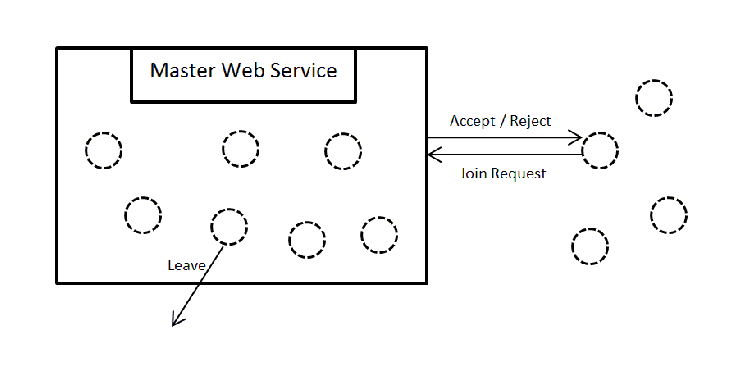
\includegraphics[width=3in]{Figures/s1.eps}`
\caption{Web Services and A Grand Community}
\label{fig_sim1}
\end{figure}

The membership decision is made based on throughput and \emph{QoS}
of the considered web service. The goal is to have quality web
services in the community so it stays stable and no other web
services would have incentives to deviate and leave the coalition
$C$. Therefore, a basic method would be to check the core of the
coalition $C$ considering all the current community members (all
web services already residing within the community) and the new
web service. This algorithm uses the \emph{Shapley value}
distribution method as described in Equation \ref{eq:shapley} to
distribute the gain of $v(C)$ among all the members and then
checks if the \emph{Shapley value} payoff vector for this
community having the characteristic function $v(C)$ is in the
\emph{core}. In the \emph{Shapley value} payoff vector, the payoff
for each web service $ws_i$ is calculated based on its marginal
contribution $v(C \cup {i}) - v(C)$ over all the possible
different permutations in which the coalition can be formed, which
makes the payoff distribution fair. Because of going through all
the possible permutations of subsets of $N$, the nature of the
\emph{Shapley value} is combinatorial, which makes it impractical
to use as the size of our coalitions grows. However, it is proven
that in convex games, the \emph{Shapley value} lies in the core
\cite{DBLP:conf/ijcai/GrecoMPS11, myerson1991game}. Thus, if the
\emph{Core} is non-empty, the payoff vector is a member of the
\emph{Core}. The following proposition is important to make our
algorithm tractable.
% so in our algorithm we check the core membership of this payoff vector.

%\ref{eq:convex}.

%\newtheorem{theorem}{Proposition}
%\begin{theorem}[Einstein-Podolsky-Rosenberg]
\begin{theorem}\label{proposition1}
A game with a characteristic function $v$
is convex if and only if for all $S$, $T$, and $i$ where $S
\subseteq T \subseteq N \backslash \left\{i\right\}, \forall i \in
N$,
%For $\forall S \subseteq T \subseteq N \backslash \left\{i\right\}, \forall i \in N$ we have:
\begin{equation}\label{eq:convex_snow}
v(S \cup \left\{i\right\}) - v(S) \leq v (T \cup \left\{i\right\}) - v(T)
\end{equation}
\end{theorem}

%\begin{Proposition}\label{proposition} A game with a characteristic function $v$
%is convex if and only if for all $S$, $T$, and $i$ where $S
%\subseteq T \subseteq N \backslash \left\{i\right\}, \forall i \in
%N$,
%For $\forall S \subseteq T \subseteq N \backslash \left\{i\right\}, \forall i \in N$ we have:
%\begin{equation}\label{eq:convex_snow}
%v(S \cup \left\{i\right\}) - v(S) \leq v (T \cup \left\{i\right\}) - v(T)
%\end{equation}
%\end{Proposition}

\begin{proof}
We first prove the ``only if'' direction:
%\\$~~~~$\textbf{1}. ``only if'' direction:\\
\\$~~~~$\ \textbf{1}. ``only if'' direction:\\
%\setlength{\abovedisplayshortskip}{2pt}
Assume:\\
\vspace{-0.5cm}
\begin{gather*}\label{convexsnowproof}
v(S \cup \left\{i\right\}) - v(S) \leq v (T \cup \left\{i\right\})
- v(T)
\\
\rightarrow v(S \cup \left\{i\right\}) + v(T) \leq v (T \cup \left\{i\right\}) + v(S)
\end{gather*}

Considering $S \subseteq T$:
\setlength{\abovedisplayshortskip}{2pt}
\begin{gather*}
S \cup \left\{i\right\} = (S \cup \left\{i\right\}) \cup T
\\
T = (S \cup \left\{i\right\}) \cap T
\end{gather*}

By setting $A = S \cup \left\{i\right\}$ and $B = T$ we have:
\setlength{\abovedisplayshortskip}{2pt}
\begin{gather*}
v(S \cup \left\{i\right\}) + v(T) \leq v (T \cup \left\{i\right\}) + v(S)
\\
\rightarrow v(S \cup \left\{i\right\}) + v(T) \leq
\\
v((S \cup \left\{i\right\}) \cup T) + v((S \cup \left\{i\right\}) \cap T)
\\
\rightarrow v(A) + v(B) \leq v(A \cup B) + v(A \cap B)
\end{gather*}
Consequently, the game is convex.

\textbf{2}. ``if'' direction:\\
Assume the game is convex. Thus, for all $A, B \subset N$, we
have: \setlength{\abovedisplayshortskip}{2pt}
\begin{gather*}
v(A) - v(A \cap B) \leq v(A \cup B) - v(B)
\end{gather*}

By setting $S \cup \left\{i\right\} = A$ and $T = B$ where $S \subseteq T$:
\setlength{\abovedisplayshortskip}{2pt}
\begin{gather*}
v(S \cup \left\{i\right\}) - v((S \cup \left\{i\right\}) \cap T) \leq v(T \cup (S \cup \left\{i\right\})) - v(T)
\\
\rightarrow v(S \cup \left\{i\right\}) - v(S) \leq v(T \cup \left\{i\right\}) - v(T)
\end{gather*}

\end{proof}

Thus, in order to keep the characteristic function convex, new web
services should have more marginal contribution as the coalition
size grows.

Our algorithm works as follows. We have an established community
with a master and some member web services already residing in the
community. A web service would send a join request to the
community. The ideal solution would be analyzing the \emph{core}
or \emph{$\epsilon$-core} stability of the group having this new
member. As the normal core membership algorithm is computationally
intractable, we exploit Proposition \ref{proposition1} and Equation
\ref{eq:convex_snow} to check the convexity of our game having
characteristic function where the new member is added. In the
equation, we set $C$ to be our community members $(C)$ before
having the new web service. We assign ${i}$ to the new web
service, and then verify the equation for $S$, setting $ S = T /
W1 $ where $W1$ is the set of all possible subsets of the set $N$
having the size $1$. We can relax the equation a bit by adding a
constant $\epsilon$ to the left side of the equation. We call this
method \emph{Depth-1 Convex-Checker} algorithm. If the equation is
satisfied for all $W1$, we let the new web service join our
community, since the web service will contribute positively enough
to make our new community stable. Since only subsets of size $1$
are checked, the following Proposition holds.

\begin{theorem}\label{complexity1}
\emph{The run time complexity of Depth-1 Convex-Checker algorithm is
$O(n)$.}
\end{theorem}

By this result, we obtain a significant reduction from $O(2^n)$,
which is the complexity of checking all possible subsets of $N$.
In our second method, we use the same algorithm, but this time we
set $W2$ to be the set of all possible subsets of size two and one
of the community $C$. We call this method \emph{Depth-2
Convex-Checker} and its run time complexity is still
linear:

\begin{theorem}\label{complexity2}
\emph{The run time complexity of Depth-2 Convex-Checker algorithm is
$O(n^2)$.}
\end{theorem}

It is possible to develop an anytime algorithm by continuing the
verification of this condition against all subsets of size $3$,
$4$, etc. until the algorithm gets interrupted.

\subsection {Web Services and Many Communities}

In this scenario, we consider multiple communities managed by
multiple master web services, each of which is providing
independent request pools (see Figure \ref{fig_sim2}). Identical
to the first scenario, master web services form coalitions with
web services. We use coalition structure formation methods to
partition web services into non-empty disjoint coalition
structures. As mentioned in Section \ref{sec:coalition}, the used
algorithms \cite{Sandholm1999209,DBLP:conf/ijcai/GrecoMPS11,DBLP:conf/ijcai/RahwanMJ11} try to
solve key fundamental problems of what coalitions to form, and how
to divide the payoffs among the collaborators.

\begin{figure}[!t]
\centering
\includegraphics[width=3in]{Figures/s2.eps}
\caption{Web Services and Many Communities}
\label{fig_sim2}
\end{figure}